%%%%%%%%%%%%%%%%%%%%%%%%%%%%%%%%%%%%%%%%%%%%%%%%%%%%%%%%%%%%%%%%%%%%%%%%%%%%%%%
%% StuPro A, Produktlinien (Kobold)
%% Team Werkbold
%% Entwurf
%% $Id: entwurf.tex,v 1.4 2004/03/22 22:03:39 rendgeor Exp $
%%%%%%%%%%%%%%%%%%%%%%%%%%%%%%%%%%%%%%%%%%%%%%%%%%%%%%%%%%%%%%%%%%%%%%%%%%%%%%%
\documentclass[a4paper,titlepage,12pt,ngerman]{scrbook}
\usepackage{../common/header}
\usepackage{supertabular}

\RCSdef $Revision: 1.4 $
\RCSdef $Date: 2004/03/22 22:03:39 $

%\newcommand\version{Version \today \xspace}
\newcommand\version{Version 1.0\xspace}

\title {\huge \product\\[0.5cm]\large Spezifikation I \\[0.5cm] \version
  \\[1cm] \Large \company}

\begin{document}

%%%%%%%%%%%%%%%%%%%%%%%%%%%%%%%%%%%%%%%%%%%%%%%%%%%%%%%%%%%%%%%%%%%%%%%%%%%%%%%
%% Deckblatt

\begin{titlepage}
\renewcommand{\thefootnote}{\fnsymbol{footnote}}
{\Huge
\raggedright
\textbf{\bf Kobold} \\
\huge Produktlinien Management System
\rule{\textwidth}{0.75pt}
\par
}
\begin{flushleft}
\normalsize
\version
\end{flushleft}


\vfill

\includegraphics[width=15cm]{../common/logo-color.png}
\vfill
{\parindent=0cm
\Huge Entwurf I
}


\setcounter{footnote}{0}
\end{titlepage}

%%%%%%%%%%%%%%%%%%%%%%%%%%%%%%%%%%%%%%%%%%%%%%%%%%%%%%%%%%%%%%%%%%%%%%%%%%%%%%%
%% Versionsgeschichte

\section*{Versionsgeschichte}

\begin{itemize}

\item Version 1.0 (21.03.2004)
    
    Diese Version wird nur intern verwendet.

\end{itemize}

%%%%%%%%%%%%%%%%%%%%%%%%%%%%%%%%%%%%%%%%%%%%%%%%%%%%%%%%%%%%%%%%%%%%%%%%%%%%%%%
%% Inhaltsverzeichnis
\tableofcontents
%%%%%%%%%%%%%%%%%%%%%%%%%%%%%%%%%%%%%%%%%%%%%%%%%%%%%%%%%%%%%%%%%%%%%%%%%%%%%%%%%%% 
\chapter{Einleitung}

\section{�ber dieses Dokument}

Diese Spezifikation dient als Grundlage zur informalen
Beschreibung des Produktlinien Management Systems \product.
Aufgrund des evolution�ren Vorgehensmodells wird dieses Dokument
iterativ erweitert und verfeinert und zu Beginn jeder
Folge-Iteration der weiteren Entwicklung zugrundegelegt.\par Das
Dokument richtet sich sowohl an den Auftraggeber und dessen
technische Berater als auch an die Mitarbeiter des
Werkbold-Teams.\par Es wird vom Auftraggeber am Anfang jeder
Iteration abgenommen und ist von da an Vertragsbestandteil f�r die
weitere Entwicklung von \product.

\subsection{Spezifikation I}
Die Spezifikation I dient als Grundlage zur informalen
Beschreibung des Rahmensystems von \product, das in der ersten
Iteration entwickelt wird.\par Sie basiert auf der Abstraktion der
ermittelten Anforderungen an das Produktlinien Management System
\product (vgl. Anhang B).\par Aufgrund des abstrakten Charakters
der Spezifikation des Rahmensystems wird auf eine explizite
Spezifikation von Use-Cases verzichtet. Diese wird Gegenstand der
Spezifikationen in den Folge-Iterationen sein.

\section{Das Kobold-System}

Das wesentliche Einsatzziel des Produktlininen Management Systems
\product ist die werkzeugunterst�tzte Entwicklung und Pflege von
Software-Produktlinien und die Etablierung eines rollenbasierten
Entwicklungsprozesses.


\subsection{Grundlegende Architekturentscheindungen}
Die grundlegende Architektur von \product untergliedert sich in
zwei Teilsysteme: der Kobold Client, der als rollenbasierte
Entwicklungsumgebung f�r die Verwaltung von Produktlinien und
Produkten konzipiert ist, und dem Kobold Server-Dienst, der die
Benutzer-, Rollen- und Nachrichten-Verwaltung erm�glicht. \par Der
Eclipse-basierte Client bietet dem Benutzer eine graphische
Benutzungsoberfl�che, �ber die er seine Produktlinien und Produkte
rollenabh�ngig verwalten kann. Er kann damit seine Architekturen
als Graphen ansehen und ver�ndern, neue Rollen verteilen,
Nachrichten verschicken und Workflows ausl�sen.\par Der Server
verwaltet die Daten der einzelnen Benutzer und deren
Zugriffsrechte. Er bietet den Clients au�erdem einen zentralen
Nachrichtendienst an. Wenn von einem Client eine Nachricht an den
Serverdienst gesendet wird, pr�ft der Serverdienst die Nachricht
auf m�gliche Konsequenzen, die anderen Clients in Form von
Workflows zugeteilt werden. Dar�ber hinaus verwaltet der
Serverdienst auch die Pfade und Zugriffskonfigurationen der
Repositories, in denen die Daten der Produkte und Produktlinien
gespeichert und versioniert werden.

\chapter{Der Kobold Client}
Der Client basiert grundlegend auf der Eclipse Plattform und deren Widgettoolkit und ist
dadurch von dessen nativer Schnittstelle abh�ngig. Laut dem Eclipse Consortium werden die folgenden 
Plattformen und Betriebssysteme unterst�tzt:
\begin{itemize}
    \item Windows NT/2000/XP
    \item Linux (x86/Motif)
    \item Linux (x86/GTK 2)
    \item Solaris 8 (SPARC/Motif)
    \item QNX (x86/Photon)
    \item AIX (PPC/Motif) 
    \item HP-UX (HP9000/Motif)
    \item Mac OSX (Mac/Carbon)
\end{itemize}
Er wird als Feature-Set implementiert und mit eigenem Product Branding versehen.
Das Product Branding umfasst die �nderung der Fensternamen und der Produkticons, sowie
einer Willkommensseite die einen kurzen �berblik �ber Funktionalit�t und Zweck des Kobold Tools geben soll.

Das Feature-Set wird als Set von inernationalisierbaren Eclipse Plugins implementiert.
Die Ausgangsperspektive wird aus 4 Teilen bestehen:
\begin{itemize}
	\item Der Produktlinienarchitektur View/Editor
	\item Der Rollen View
	\item Der Worklflow/Task View
	\item Die Minimap
\end{itemize}
Diese werden in den jeweiligen Unterkapiteln n�her beschrieben.
Um das Rollenprinzip konsistent durchzusetzen ist eine zentrale Anmeldung an einem Server n�tig.
Details zu der Serverseitigen L�sung finden sie auf Seite %todo Link zur Serverseite% 
. 
\section{Authentifizierung}
Die Authentifizierung am Server erfolgt durch einen RPC. Der Benutzer kann bei der Erstbenutzung des 
Clients w�hlen ob er sich bei jedem Programmstart authentifiziern will, oder ob das Passwort
und der Benutzername gespeichert werden sollen. Prinzipiell ist ein �ndern von Daten im nichtauthentifizierten
Zustand nicht m�glich. Mit der Authentifizierung werden die Rollen die dem Benutzer zugeteilt sind,
an den Client �bergeben, der Client reagiert seinerseits mit dem Bereitstellen der relevanten Sichten/
Views f�r den Benutzer.
\section{Der Produktlinienarchitektur View/Editor}
In diesem View wird die je nach aktiver Rolle relevante Sicht auf die Architektur der Produktlinie
angezeigt. Die grafische "Notation" h�lt sich dabei an die in dem Paper ... festgelegte Struktur.
Um dies nocheinmal grafisch darzustellen hier noch einmal die 3 verschiedenen Sichten auf die
Produktlinien bzw. Produktarchitektur.
Die Ansicht bietet die M�glichkeit verschidene Zoomstufen einzustellen. Dies reultiert darin,
dass im aktuellen Ausschnitt m�glicherweise nicht die ganze Architektur zu sehen ist.
Um trotzdem den �berblick zu gew�hrleisten wird eine Minimap zur Verf�gung gestellt.

%todo Grafiken einf�gen%
\subsection{Ansicht der Rolle ProduktlinienIngenieur}

\begin{figure}[ht]
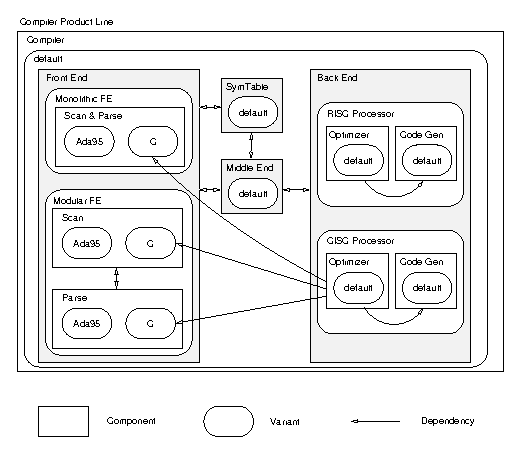
\includegraphics[width=15cm]{compiler-spl}
   \caption{Sicht des Produktlinieningenieurs}
\end{figure}
\subsection{Ansicht der Rolle eines Produktingenieurs}
\begin{figure}[ht]
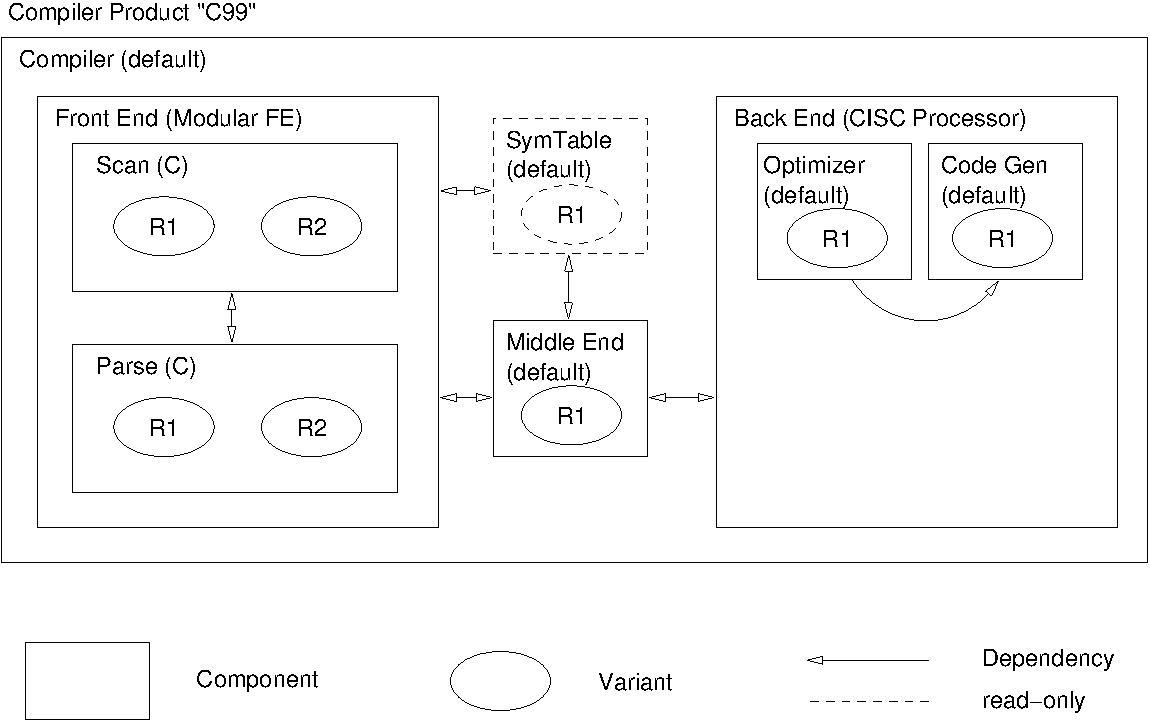
\includegraphics[width=15cm]{compiler-pe}
   \caption{Sicht des Produktingenieurs}
\end{figure}
\subsection{Ansicht der Rolle eines Programmierers}
\begin{figure}[ht]
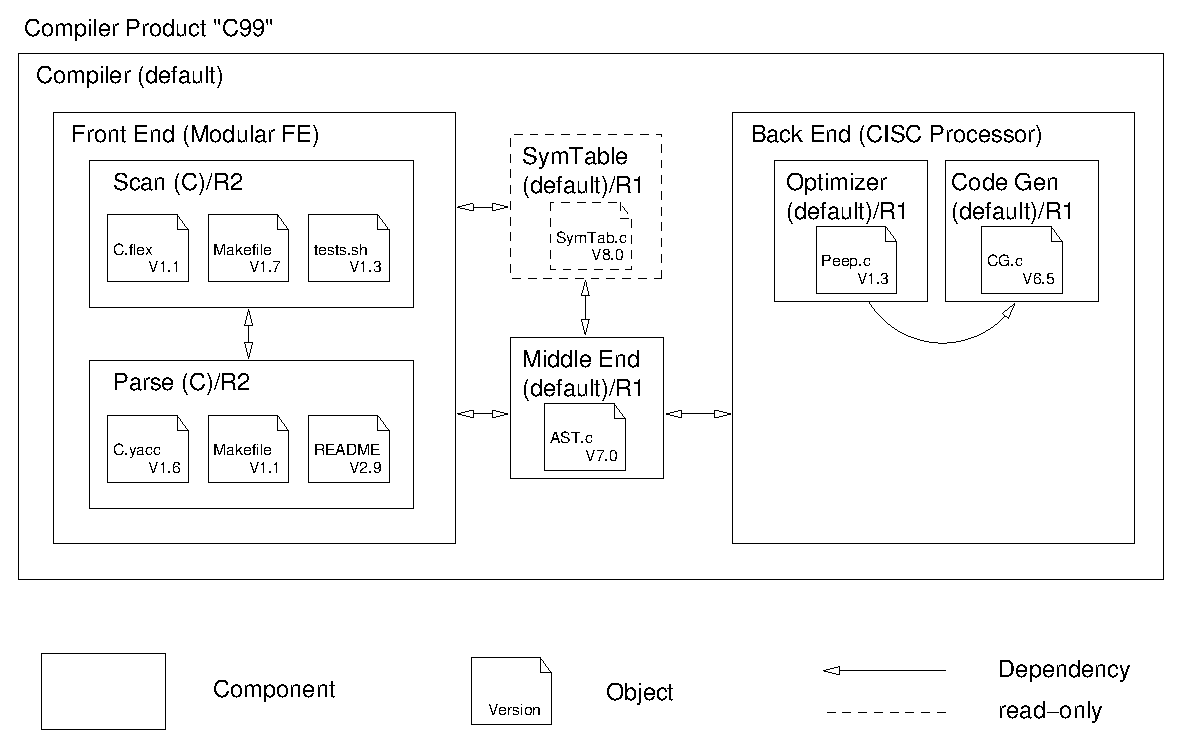
\includegraphics[width=15cm]{compiler-p}
   \caption{Sicht des Programmierers}
\end{figure}

\section{Der Rollen View}
Auf der linken Seite der Ausgangsperspektive wird ein hierarchischer Baum angezeigt, der
die momentan aktive Rolle und die mit Ihr verbundenen m�glichen Sichten darstellt.
\section{Der Worklflow/Task View}
Am unteren Rand der Ausgangsperspektive wird standardm�ssig 
\section{Die Minimap}
Am rechten unteren Rand der Ausgangsperspektive wird eine sogennante Minimap angezeigt,
in der ein �berblick �ber die ganze Architektursicht der aktuellen Rolle gegeben wird.


%%%%%%%%%%%%%%%%%
%% VCM-Wrapper (Oli)
%%%%%%%%%%%%%%%%%%%
\section{Delegater-Schicht}
\subsection{Ablauf}

Der Delegater meldet sich mit Benutzernamen und Passwort am Server an und
erh�lt vom Server eine spezifische Session-ID. Danach werden vom
Server alle Konfigurationsdaten geladen und diese automatisch in
Eclipse gespeichert.

\subsection{Automatischer Login bei wiederholtem Zugriff}
Beim ersten Login am Server wird von diesem eine eindeutige Session-ID
vergeben, die bei erneutem Zugriff auf den Server zur
Authentifizierung genutzt wird. Damit ist gemeint, dass dadurch das
erneute eingeben des Benutzernamens und des Passwort nicht notwendig
ist.\par
Falls der Server bemerkt, dass die selbe Session-ID zur
Authentifizierung von 2 verschiedenen Clients verwendet wird, wird
diese ung�ltig. Als folge dessen muss sich der Benutzer erneut mit
Benutzernamen und Passwort authentifizieren und erh�lt eine neue
Session-ID. Daher sollte beim Arbeiten eines Benutzers von verschieden
Client-Rechner unbedingt f�r jeden Arbeitsplatz eine eigene Session-ID
benutzt werden.

\subsection{R�ckgabewerte des Servers}
Durch die Auswertung der R�ckgabewerte kann die Delegater-Schicht
entscheiden, ob die Server-Aktion erfolgreich ausgef�hrt wurde.

\section{Controlerkomponente VCM-Wrapper}
\subsection{Zusammenfassung}
Der VCM-Wrapper spiegelt der Eclipse-Plattform ein vollfunktionsf�higes Team-
Plugin vor, �ber das alle Repositoryoperationen durchgef�hrt werden. Intern
gibt die Komponente die Aktionen jedoch an andere Team-Plugins weiter. Vor und
nach jeder dieser Aktion wird die Kommunikations-Komponente konsultiert, um 
den Server bzw. andere Clients �ber Ver�nderungen am Repository zu 
informieren. Die VCM-Wrapper-Komponente kennt sowohl die Datei-Ebene und deren
Repositories als auch die Abstraktion auf Produktlinien/Komponenten/Varianten.
F�r beide Ebenen lassen sich atomare (z.B. checkin) und komplexe VCM-
Aktionen () ausf�hren. Die n�tigen Informationen �ber 
Repository-Positionen und Struktur bezieht der VCM-Wrapper �ber die Server-
Kommunikations-Komponente sowie das Architekturmodel.

%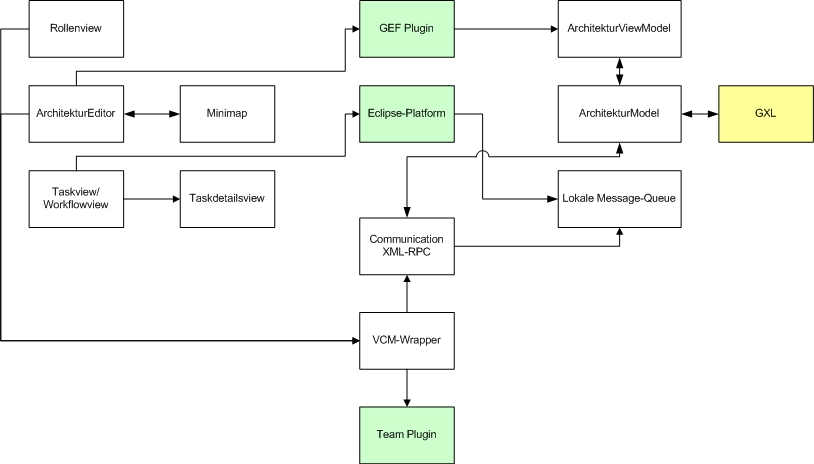
\includegraphics[width=15cm]{client.jpg}

\subsection{Manueller Import der Einstellungen}
Der Client st�� die Delegater-Schicht an. Als positives Ergebnis sind
alle Konfigurationsdaten in Eclipse gespeichert. 
\par 
Durch diese Konfigurationsdaten kann Eclipse entscheiden welche
Repositories, zugeh�rige Rollen und Zugriffsrechte benutzt werden
m�ssen.
Dadurch k�nnen in Eclipse durch die erhaltenen Rollen und
Repository-Daten die vordefinierten Felder zum Zugriff auf
VCM-Repositories entsprechend gesetzt werden. Hierdurch wird eine
optimale Anbindung an bereits existierende Eclipse-Strukturen
geschaffen. 

\subsection{Automatischer Import der Einstellungen}
Falls der Benutzer das erste Mal Eclipse startet, d.h. noch keine
Konfigurationsdaten zu Rollen und Repositories vorliegen, wird die
delegater-Schicht automatisch angesto�en, und die Konfigurationsdaten
vom Server geladen und in Eclipsae gepeichert, wie im manuellen
Import n�her beschrieben.

\subsection{Ablaufschritte beim Zugriff auf das Repository}

Die Ablaufschritte:\par

\begin{itemize}
    \item Lade Konfigurationsdaten vom Server (fetch)
    \item Extrahiere Rollenzuteilung, Repository-Daten
    \item Lokale Pr�fung auf vorhandenes Produkt, d.h. Produktdaten, Benutzerdaten (check)
    \item Pr�fungsergebnisse f�hren bei nicht vorhandenem Produkt zu
    �ffnendem Dialog und anschlie�ender Lade-Aktion (checkout) aus dem
    Repository
\end{itemize}\par

\subsection{M�gliche Wrapper-Aktionen}

Alle m�glichen Wrapper-Aktionen lassen sich in zwei verschiedene
Gruppen einteilen. Aktionen die keine Berechtigung erfordern, d.h. f�r
alle Benutzer m�glich sind und Aktionen die eine Berechtigung
erfordern, d.h. nur f�r bestimmte m�glich sind.\par

Die sichtbaren Aktionen:\par

{\bf Alle Benutzer:}
\begin{itemize}
  \item check out: immer m�glich, ggf. nur Leserechte.
  \item update: Vorbedingung: check out
\end{itemize}

{\bf Nur bestimmte Benutzer:}

\begin{itemize}
  \item commit: Vorbedingung: check out
  \item import: in der ersten Iteration nicht m�glich!
  \item delete: -
  \item add: -
\end{itemize}

Falls eine Aktion der zweiten Gruppe nicht erfolgreich ausgef�hrt
werden kann, entweder weil der Client feststellt dass der Benutzer
nicht die passende Rolle besitzt, d.h. eine unerlaubte Aktion
angesto�en wurde oder weil der Repository-Server beim durchf�hren der
Aktion eine Fehlermeldung zur�ck gibt wird auf dem Server ein
passender Workflow der zu dem speziellen Feedback passt, angestossen.


\subsection{Skriptausf�hrung}
Allen m�glichen Wrapper-Aktionen kann zus�tzlich eine bestimmte
Matainfo-Datei �bergeben werden, das eine georndete Liste von Skripten
enth�lt, die vor und nach einem ``commit'' ausgef�hrt werden. Diese
m�glichen Metainfo-Dateien werden an anderer Stelle festgelegt.

\subsection{Der (initiale) Metadaten-Abgleich}
{\bf Vorbedingung:} Um einen korrekten Konsistenzcheck durchf�hren zu
k�nnen, m�ssen Informationen �ber alle Dateien, Verzeichnisse, deren
Autoren und die vorhandenen Dateiversionen vorliegen. Diese werden im
weiteren als Metadaten bezeichnet.\par
Da es passieren kann, dass verschiedene Personen an Dateien und
Versionen arbeiten, sollte vor der produktzusammenstellung eine
erneute Syncronisation dieser Daten durchgef�hrt werde.

\subsection{Reihenfolge beim Schreiben von Metainformationen}
\begin{itemize}
  \item commit aller Dateien (�nderungen)
  \item update des Repositories, damit werden die aktuellen (neuen)
  Revisionsnummern gesetzt)
  \item commit der Metadaten (neue Revisionen)
\end{itemize}


\subsection{Konsistenzcheck bei der Produktzusammenstellung}
Als Konsistenzcheck wird die Anfrage an die Datenbasis genannt, die
als Eingabeparameter die Revision oder den Autor einer bestimmten
Datei xy erh�lt und zur�ckgibt, ob die Datei vorhanden (match=syncron)
ist (oder nicht) und ob die Revision �bereinstimmt. Im Fehlerfall wird
ein passender Workflow angesto�en.\par
Zur �berpr�fung des gesamten Produktes werden oben genannte Schritte
angewandt, wobei die Eingabemenge aus Dateinamen und deren Revisionen
besteht.


\subsection{Einschr�nkungen bei der Implementierung}
\begin{itemize}
  \item ``eigene'' Eclipse VCM-Aktionen m�ssen abgefangen
  werden. Ansonsten k�nnen Daten ungesehen manipuliert
  werden. Ggf. erlauben, aber dann den Benutzer auf die Folgen
  hinweisen.
  \item ``eigene'' eclipse VCM-Aktionen sind nur �ber ``Extension
  Points'' aufrufbar, daher muss im ``red book'' nach guten
  Code-Schnittstellen geschaut werden.
  \item
\end{itemize}




\chapter{Server}

Dieser Abschnitt beschreibt die Komponenten des Entwurfs des
Kobold Servers. In der Iteratrion 1 untergliedert sich der Server
in 5 Komponenten. Man beachte insbesondere auch das Kapitel 2.3
der Spezifikation1, das die Anforderungen an die jeweiligen
Komponenten spezifiziert.

\section{�berblick}
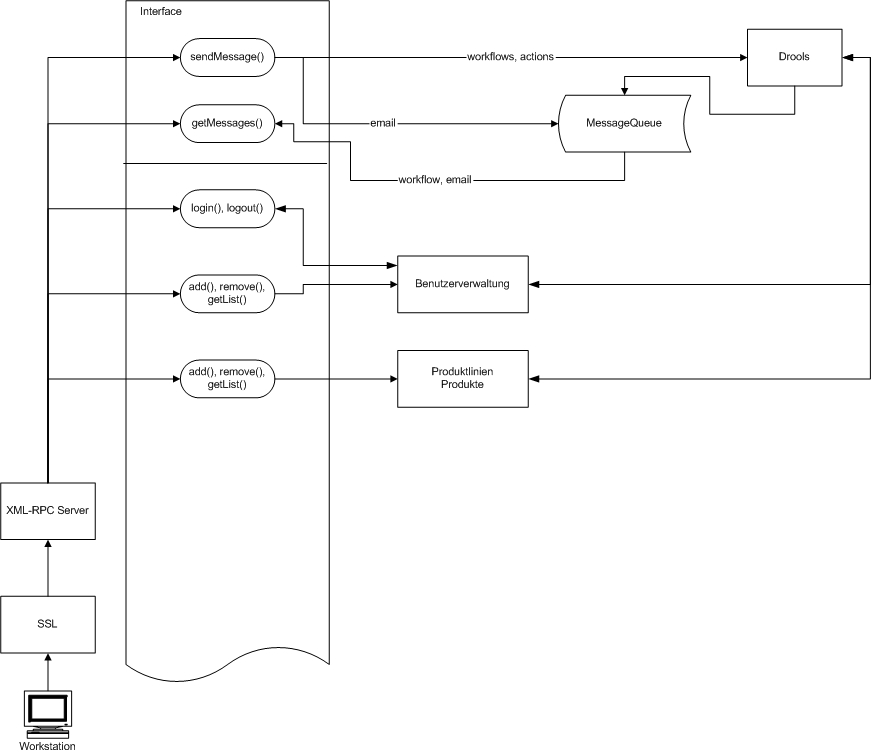
\includegraphics[width=15cm]{server.jpg}

\section{Komponente Kobold Interface}

Die Komponente Interface bildet die Schnittstelle des Kobold
Servers nach aussen und ist dessen Einsprungklasse. Sie wird von
den Kobold Clients �ber remote procedure calls angesprochen.
Anfragen werden an die daf�r zust�ndigen Komponenten des Kobold
Servers delegiert.

\section{Komponente WorkflowEngine}

Diese Komponente erh�lt Daten �ber durchgef�hrte (VCM-)Actionen
sowie Workflowobjekte, die auf die vorhandenen Regelmengen
angewendet werden. Daf�r k�nnen ben�tigte Daten von den
Komponenten Benutzerverwaltung und Produktlinienverwaltung
abgerufen werden. Als Konsequenz k�nnen Workflows oder EMails an
die MessageQueue-Komponente �bergeben werden.

\section{Komponente MessageQueue}

Aufgabe dieser Komponente ist die Verwaltung und Zustellung von
Worklows und EMails an die addressierten Clients, sobald diese
getMessages() aufrufen.

\section{Komponente Benutzerverwaltung}

Die Benutzerverwaltung ist zust�ndig f�r die Authentifizierung der
Benutzer beim Login und verwaltet deren Rollendaten. S�mtliche
Benutzerdaten k�nnen von dieser Komponente abgefragt werden.

\section{Komponente Produktlinien-/Produktverwaltung}

Diese Komponente verwaltet s�mtliche auf dem Server zu
persistierende Daten zu Produktlinien und Produkten.

\chapter{Interface} \label{cha_interface}
Die Kommunikation zwischen Client und Server erfolgt via XML-RPC. 
Dazu muss auf beiden Seiten eine Schnittstelle definiert sein.

\section{Synchrone Kommunikation}
Die synchrone Kommunikation dient der direkten Abfrage des Servers sowie zum
An- und Abmelden des Clients bzw. des Benutzers.

Folgende Methoden sind definiert:\par

\subsection{Authentifizierung}
\verb+/**+\\
\verb+ * Anmelden eines Benutzers.+\\
\verb+ * Der Benutzer wird authentifiert und es wird eine Session angelegt.+\\
\verb+ *+\\
\verb+ * @param username - Benutzername+\\
\verb+ * @param password - Passwort+\\
\verb+ *+\\
\verb+ * @return mixed   - Gemischte Datenstruktur, enth�lt Informationen+\\
\verb+ *                   �ber den Benutzer, dessen Rollen, Produktlinien+\\
\verb+ *                   und Produkten denen er angeh�rt.+\\
\verb+ *                   Ausserdem wird die Session-ID zurueckgegeben.+\\
\verb+ *                   Ein Fehlschlag der Authentifizierung gibt false.+\\
\verb+ *                   zur�ck.+\\
\verb+ */+\\
\verb+mixed login(String username, String password)+\\

\verb+/**+\\
\verb+ * Abmelden eines Benutzers.+\\
\verb+ * Der Benutzer wird abgemeldet und die Session zerst�rt.+\\
\verb+ *+\\
\verb+ * @param sessionId - SessionId+\\
\verb+ *+\\
\verb+ */+\\
\verb+void logout(String sessionId)+\\

\subsection{Benutzerverwaltung}
\verb+/**+\\
\verb+ * Hinzuf�gen eines Benutzers.+\\
\verb+ *+\\
\verb+ * @param sessionId - SessionId+\\
\verb+ * @param info      - Benutzerinformationen+\\
\verb+ *+\\
\verb+ * @return boolean  - Erfolgreich?+\\
\verb+ */+\\
\verb+boolean addUser(String sessionId, mixed info)+\\

\verb+/**+\\
\verb+ * Entfernen eines Benutzers.+\\
\verb+ *+\\
\verb+ * @param sessionId - SessionId+\\
\verb+ * @param username  - Benutzername+\\
\verb+ *+\\
\verb+ * @return boolean  - Erfolgreich?+\\
\verb+ */+\\
\verb+boolean removeUser(String sessionId, String username)+\\

\verb+/**+\\
\verb+ * Abfrage eines Benutzers.+\\
\verb+ *+\\
\verb+ * @param sessionId - SessionId+\\
\verb+ * @param username  - Benutzername+\\
\verb+ *+\\
\verb+ * @return mixed    - Benutzerinformationen+\\
\verb+ */+\\
\verb+mixed getUser(String sessionId, String username)+\\

\verb+/**+\\
\verb+ * Modifizieren eines Benutzers.+\\
\verb+ *+\\
\verb+ * @param sessionId - SessionId+\\
\verb+ * @param username  - Benutzername+\\
\verb+ * @param info      - Benutzerinformationen+\\
\verb+ *+\\
\verb+ * @return boolean  - Erfolgreich?+\\
\verb+ */+\\
\verb+boolean modifyUser(String sessionId, String username, mixed info)+\\

\verb+/**+\\
\verb+ * Liste der Benutzer abfragen.+\\
\verb+ *+\\
\verb+ * @param sessionId - SessionId+\\
\verb+ *+\\
\verb+ * @return list     - Liste aller Benutzernamen+\\
\verb+ */+\\
\verb+list getUsers(String sessionId)+\\

\subsection{Produktlinienverwaltung}
\verb+/**+\\
\verb+ * Hinzuf�gen einer Produktlinie.+\\
\verb+ *+\\
\verb+ * @param sessionId - SessionId+\\
\verb+ * @param info      - Produktlinieninformationen+\\
\verb+ *+\\
\verb+ * @return boolean  - Erfolgreich?+\\
\verb+ */+\\
\verb+boolean addProductline(String sessionId, mixed info)+\\

\verb+/**+\\
\verb+ * Entfernen einer Produktlinie.+\\
\verb+ *+\\
\verb+ * @param sessionId    - SessionId+\\
\verb+ * @param productline  - ProduktlinienID+\\
\verb+ *+\\
\verb+ * @return boolean     - Erfolgreich?+\\
\verb+ */+\\
\verb+boolean removeProductline(String sessionId, String productline)+\\

\verb+/**+\\
\verb+ * Abfrage einer Produktlinie.+\\
\verb+ *+\\
\verb+ * @param sessionId    - SessionId+\\
\verb+ * @param productline  - ProduktlinienID+\\
\verb+ *+\\
\verb+ * @return mixed       - Produktlinieninformationen+\\
\verb+ */+\\
\verb+mixed getProductline(String sessionId, String productline)+\\

\verb+/**+\\
\verb+ * Modifizieren einer Produktlinie.+\\
\verb+ *+\\
\verb+ * @param sessionId    - SessionId+\\
\verb+ * @param productline  - ProduktlinienID+\\
\verb+ * @param info         - Produktlinieninformationen+\\
\verb+ *+\\
\verb+ * @return boolean     - Erfolgreich?+\\
\verb+ */+\\
\verb+boolean modifyProductline(String sessionId, String productline,+\\
\verb+                                            mixed info)+\\
\verb+/**+\\
\verb+ * Liste der Produktlinien abfragen.+\\
\verb+ *+\\
\verb+ * @param sessionId - SessionId+\\
\verb+ *+\\
\verb+ * @return list     - Liste aller Produktlinien+\\
\verb+ */+\\
\verb+list getProductlines(String sessionId)+\\

\verb+/**+\\
\verb+ * Benutzer zu der Produktlinie hinzuf�gen.+\\
\verb+ *+\\
\verb+ * @param session     - SessionId+\\
\verb+ * @param productline - ProduktlinienId+\\
\verb+ * @param user        - BenutzerId+\\
\verb+ */+\\
\verb+void addUserToPL(String sessionId, String productline, String user)+\\

\verb+/**+\\
\verb+ * Benutzer von der Produktlinie entfernen.+\\
\verb+ *+\\
\verb+ * @param session     - SessionId+\\
\verb+ * @param productline - ProduktlinienId+\\
\verb+ * @param user        - BenutzerId+\\
\verb+ */+\\
\verb+void removeUserFromPL(String sessionId, String productline,)+\\
\verb+                                        String user)+\\

\verb+/**+\\
\verb+ * Liste der Produktlinien-Benutzer abfragen.+\\
\verb+ *+\\
\verb+ * @param sessionId   - SessionId+\\
\verb+ * @param productline - ProduktlinienId+\\
\verb+ *+\\
\verb+ * @return list       - Liste aller Produktlinienbenutzer+\\
\verb+ */+\\
\verb+list getPLUsers(String sessionId, String productline)+\\



\subsection{Produktverwaltung}
\verb+/**+\\
\verb+ * Hinzuf�gen eines Produkts zu einer Produktlinie.+\\
\verb+ *+\\
\verb+ * @param sessionId   - SessionId+\\
\verb+ * @param productline - ProduktlinienID+\\
\verb+ * @param info        - Produktinformationen+\\
\verb+ *+\\
\verb+ * @return String     - ProduktID+\\
\verb+ */+\\
\verb+String addProduct(String sessionId, String productline, mixed info)+\\

\verb+/**+\\
\verb+ * Entfernen eines Produkts aus einer Produktlinie.+\\
\verb+ *+\\
\verb+ * @param sessionId   - SessionId+\\
\verb+ * @param productline - ProduktlinienID+\\
\verb+ * @param product     - ProduktID+\\
\verb+ *+\\
\verb+ * @return boolean    - Erfolgreich?+\\
\verb+ */+\\
\verb+boolean removeProduct(String sessionId, String productline,)+\\
\verb+                                        String product)+\\

\verb+/**+\\
\verb+ * Abfrage eines Produkt.+\\
\verb+ *+\\
\verb+ * @param sessionId - SessionId+\\
\verb+ * @param product   - ProduktID+\\
\verb+ *+\\
\verb+ * @return mixed    - Produktlinieninformationen+\\
\verb+ */+\\
\verb+mixed getProduct(String sessionId, String product)+\\

\verb+/**+\\
\verb+ * Modifizieren eines Produkts.+\\
\verb+ *+\\
\verb+ * @param sessionId - SessionId+\\
\verb+ * @param product   - ProduktID+\\
\verb+ * @param info      - Produktinformationen+\\
\verb+ *+\\
\verb+ * @return boolean  - Erfolgreich?+\\
\verb+ */+\\
\verb+boolean modifyProduct(String sessionId, String product, mixed info)+\\

\verb+/**+\\
\verb+ * Liste der Produkte abfragen.+\\
\verb+ *+\\
\verb+ * @param sessionId   - SessionId+\\
\verb+ * @param productline - ProduktlinienID+\\
\verb+ *+\\
\verb+ * @return list       - Liste aller Produkte in der Produktlinie+\\
\verb+ */+\\
\verb+list getProducts(String sessionId, String productline)+\\


\verb+/**+\\
\verb+ * Benutzer zu dem Produkt hinzuf�gen.+\\
\verb+ *+\\
\verb+ * @param session - SessionId+\\
\verb+ * @param product - ProduktId+\\
\verb+ * @param user    - BenutzerId+\\
\verb+ */+\\
\verb+void addUserToP(String sessionId, String product, String user)+\\

\verb+/**+\\
\verb+ * Benutzer von dem Produkt entfernen.+\\
\verb+ *+\\
\verb+ * @param session - SessionId+\\
\verb+ * @param product - ProduktId+\\
\verb+ * @param user    - BenutzerId+\\
\verb+ */+\\
\verb+void removeUserFromP(String sessionId, String product, String user)+\\

\verb+/**+\\
\verb+ * Liste der Produkt-Benutzer abfragen.+\\
\verb+ *+\\
\verb+ * @param sessionId - SessionId+\\
\verb+ * @param product   - ProduktId+\\
\verb+ *+\\
\verb+ * @return list       - Liste aller Produktbenutzer+\\
\verb+ */+\\
\verb+list getPUsers(String sessionId, String product)+\\

\section{Asynchrone Kommunikation}
Die asynchrone Kommunikation wird zum Datenaustausch zwischen den Clients
verwendet. Es werden Nachrichten/Workflows an den Server gesendet und in die 
MessageQueue einsortiert. Die betreffenden Clients holen sich die Nachricht
dort ab.

Folgende Methoden sind definiert:\par

\verb+/**+\\
\verb+ * Nachricht/Workflow/Aktion versenden.+\\
\verb+ * Zieladressen etc. werden mit in das Message-Object kodiert.+\\
\verb+ *+\\
\verb+ * @param session - SessionId+\\
\verb+ * @param message - Nachricht/Aktion/Workflow+\\
\verb+ */+\\
\verb+void sendMessage(String sessionId,  mixed message)+\\

\verb+/**+\\
\verb+ * Nachrichten abfragen.+\\
\verb+ * Es werden alle Nachrichten von der MessageQueue des Benutzers+\\
\verb+ * an den Client �bertragen. Die Nachrichten werden danach von+\\
\verb+ * der MessageQueue gel�scht.+\\
\verb+ *+\\
\verb+ * @param sessionId - SessionId+\\
\verb+ *+\\
\verb+ * @return list     - Nachrichtenobjekte+\\
\verb+ */+\\
\verb+list getMessages(String sessionId)+\\


%%%%%%%%%%%%%%%%%%%%%%%%%%%%%%%%%%%%%%%%%%%%%%%%%%%%%%%%%%%%%%%%%%%%%%%%%%%%%%%
%% Anhang
\appendix
%%%%%%%%%%%%%%%%%%%%%%%%%%%%%%%%%%%%%%%%%%%%%%%%%%%%%%%%%%%%%%%%%%%%%%%%%%%%%%%
%% StuPro A, Produktlinien (Kobold)
%% Team Werkbold
%% Angebot
%% $Id: begriffslexikon.tex,v 1.6 2004/02/19 14:04:10 grosseml Exp $
%%%%%%%%%%%%%%%%%%%%%%%%%%%%%%%%%%%%%%%%%%%%%%%%%%%%%%%%%%%%%%%%%%%%%%%%%%%%%%%
\newcommand{\begriff}[2]
{\item \bfseries{#1} \textnormal{#2}}

\chapter{Begriffslexikon}
\begin{itemize}

\begriff{Ansicht}{Eine rollenabh�ngige Sicht}

\begriff{Arbeitskopie}{Kopie, mit der gearbeitet wird und die tats�chlich ver�ndert wird}

\begriff{Architektur}{Struktur von Software, die aus Komponenten und
Konnektoren besteht}

\begriff{Auschecken}{VCM-Funktion zum Anfordern einer Arbeitskopie aus dem Repository}

\begriff{Assets}{Wiederverwendbare Komponenten, z.B. Source-Pakete, Klassen,
usw.}

\begriff{Core-Assets}{Architekturkomponenten, die bestimmte Funktionalit�ten 
erf�llen und oft wiederverwendet werden. Sie bilden mit den produktspezifischen 
Komponenten das Produkt}

\begriff{Core-Asset-Entwickler}{Softwareentwickler, der Core-Assets entwickelt}

\begriff{Core-Asset-Repository}{Entwicklungs-Repository (Arbeitskopie) der
Core-Assets}

\begriff{Deprecated}{Veraltet, missbilligend}

\begriff{Einchecken}{VCM-Funktion zum R�ckschreiben der Arbeitskopie-�nderungen
ins Repository}

\begriff{Entwicklungs Repository} {Siehe Arbeitskopie}

\begriff{Erstentwicklung}{Entwicklung eines neuen Produkts bzw. eines neuen 
Core-Assets}

\begriff{Evolution�res Vorgehensmodell}{Inkrementelles Vorgehensmodell in der
Softwareentwicklung, �hnlich dem Spiralmodell nach B.W. Boehm}

\begriff{Fakt}{eine Mitteilung an den Kobold-Server}

\begriff{Feature-Set}{Ein Plugin-Satz zur Erweiterung von Eclipse, so dass 
Eclipse nach der Erweiterung ein eigenes Erscheinungsbild hat}

\begriff{Iteration}{Phase im evolution�ren Vorgehensmodell}

\begriff{Kernkomponenten}{siehe Core-Assets}

\begriff{Komponenten}{Bestandteile der Produktlinien- bzw. Produktarchitektur}

\begriff{Message-Queue}{Nachrichten, die auf Anfrage an den Benutzer geleitet werden}

\begriff{Metainformation}{Zusatz-Informationen �ber Informationen}

\begriff{Module}{siehe Komponenten}

\begriff{Plugin}{Softwarekomponente, die die Funktionalit�t des Systems erweitert}

\begriff{Produktarchitektur}{Software-Architektur eines Produktes}

\begriff{Produkt-Entwickler}{P, Softwareentwickler dessen Vorgesetzter ein
Produkt-Ingenieur ist}

\begriff{Produkt-Ingenieur}{PE, ein Software-Ingenieur mit Leitungs- und 
Entscheidungskompetenz bzgl. der technischen Realisierung des Produkts. 
Der PE hat den Produktlinien-Ingenieur als Vorgesetzten.}

\begriff{Produktlinien-Ingenieur}{PLE, Software-Ingenieur mit projekt�bergreifender 
Leitungs- und Entscheidungskompetenz bzgl. der technischen Realisierung 
und Pflege der Produktlinienarchitektur.}

\begriff{Produkt-Repository}{Repository, das vom PE verwaltet wird, Entwickler
checken Arbeitskopien von Produkt�Komponenten aus}

\begriff{Produktlinien-Repository}{Repository, das vom PLE verwaltet wird, PE checken
Arbeitskopien von Core-Asset Varianten aus}

\begriff{Prototyp}{Entwicklungsversion eines Programmes}

\begriff{RPC}{Remote Procedure Call erlaubt die Ausf�hrung von Funktionen, 
die auf einem anderen Rechner implementiert sind}

\begriff{Repository}{Datei-Verwaltung zur Verwaltung von Versionen}

\begriff{Softwarearchitektur}{siehe Architektur}

\begriff{Update}{VCM-Funktion, die die Arbeitskopie mit dem Repository
synchronisiert}

\begriff{Varianten}{Modifikationen von Core-Assets}

\begriff{VCM}{Version Control Management, ein Versionsverwaltungssystem wie z.B.
das Versionsverwaltungstool CVS (Concurrent Versions System)}

\begriff{Version}{Eindeutige Bezeichnung zu einem fixen Zeitpunkt}

\begriff{View}{Subfenster von Kobold-Client}

\begriff{Wasserfall-Vorgehensmodell}{Klassisches Vorgehensmodell in der
Softwareentwicklung, das in Phasen aufgeteilt ist, die aufeinander folgen}

\begriff{Workflow}{Arbeits- bzw. Gesch�ftsprozess}

\end{itemize}

%%% Local Variables: 
%%% TeX-master: "angebot"
%%% End: 
%%% vim:tw=79:


\end{document}
%%% vim:tw=79:
